\documentclass{standalone}
\usepackage{tikz}
\usepackage{ctex,siunitx}
\setCJKmainfont{Noto Serif CJK SC}
\usepackage{tkz-euclide}
\usepackage{amsmath}
\usetikzlibrary{patterns, calc}
\usetikzlibrary {decorations.pathmorphing, decorations.pathreplacing, decorations.shapes,}

\begin{document}
\small
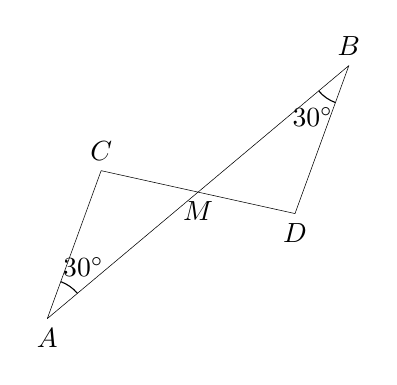
\begin{tikzpicture}[>=stealth,scale=1]
  \tkzSetUpPoint[fill=black]
  % \useasboundingbox(-1,-0.75)rectangle(3.7,1.4);
  \tkzDefPoints{0/0/A}
  \tkzDefPoint(70:2){C}
  \tkzDefPoint(40:2.5){M}
  \tkzDefPointWith[linear,K=2](A,M) \tkzGetPoint{B}
  \tkzDefPointWith[linear,K=2](C,M) \tkzGetPoint{D}
  \tkzLabelPoints[below](A,M,D)
  \tkzLabelPoints[above](B,C)
  \tkzMarkAngles[mark=none, size=.5](M,A,C M,B,D)
  \tkzDrawPolygon(M,A,C)
  \tkzDrawPolygon(M,B,D)
  \tkzLabelAngle[pos=.8](M,A,C){\ang{30}}
  \tkzLabelAngle[pos=.8](M,B,D){\ang{30}}
\end{tikzpicture}
\end{document}